% A LaTeX template for MSc Thesis submissions to 
% Politecnico di Milano (PoliMi) - School of Industrial and Information Engineering
%
% S. Bonetti, A. Gruttadauria, G. Mescolini, A. Zingaro
% e-mail: template-tesi-ingind@polimi.it
%
% Last Revision: October 2021
%
% Copyright 2021 Politecnico di Milano, Italy. NC-BY

\documentclass{Configuration_Files/PoliMi3i_thesis}

%------------------------------------------------------------------------------
%	REQUIRED PACKAGES AND  CONFIGURATIONS
%------------------------------------------------------------------------------

% CONFIGURATIONS
\usepackage{parskip} % For paragraph layout
\usepackage{setspace} % For using single or double spacing
\usepackage{emptypage} % To insert empty pages
\usepackage{multicol} % To write in multiple columns (executive summary)
\setlength\columnsep{15pt} % Column separation in executive summary
\setlength\parindent{0pt} % Indentation
\raggedbottom  

% PACKAGES FOR TITLES
\usepackage{titlesec}
% \titlespacing{\section}{left spacing}{before spacing}{after spacing}
\titlespacing{\section}{0pt}{3.3ex}{2ex}
\titlespacing{\subsection}{0pt}{3.3ex}{1.65ex}
\titlespacing{\subsubsection}{0pt}{3.3ex}{1ex}
\usepackage{color}

% PACKAGES FOR LANGUAGE AND FONT
\usepackage[english]{babel} % The document is in English  
\usepackage[utf8]{inputenc} % UTF8 encoding
\usepackage[T1]{fontenc} % Font encoding 
\usepackage[11pt]{moresize} % Big fonts

% PACKAGES FOR IMAGES
\usepackage{graphicx}
\usepackage{transparent} % Enables transparent images
\usepackage{eso-pic} % For the background picture on the title page
\usepackage{subfig} % Numbered and caption subfigures using \subfloat.
\usepackage{tikz} % A package for high-quality hand-made figures.
\usetikzlibrary{}
\graphicspath{{./Images/}} % Directory of the images
\usepackage{caption} % Coloured captions
\usepackage{xcolor} % Coloured captions
\usepackage{amsthm,thmtools,xcolor} % Coloured "Theorem"
\usepackage{float}

% STANDARD MATH PACKAGES
\usepackage{amsmath}
\usepackage{amsthm}
\usepackage{amssymb}
\usepackage{amsfonts}
\usepackage{bm}
\usepackage[overload]{empheq} % For braced-style systems of equations.
\usepackage{fix-cm} % To override original LaTeX restrictions on sizes

% PACKAGES FOR TABLES
\usepackage{tabularx}
\usepackage{longtable} % Tables that can span several pages
\usepackage{colortbl}

% PACKAGES FOR ALGORITHMS (PSEUDO-CODE)
\usepackage{algorithm}
\usepackage{algorithmic}

% PACKAGES FOR REFERENCES & BIBLIOGRAPHY
\usepackage[colorlinks=true,linkcolor=black,anchorcolor=black,citecolor=black,filecolor=black,menucolor=black,runcolor=black,urlcolor=black]{hyperref} % Adds clickable links at references
\usepackage{cleveref}
\usepackage[square, numbers, sort&compress]{natbib} % Square brackets, citing references with numbers, citations sorted by appearance in the text and compressed
\bibliographystyle{abbrvnat} % You may use a different style adapted to your field

% OTHER PACKAGES
\usepackage{pdfpages} % To include a pdf file
\usepackage{afterpage}
\usepackage{lipsum} % DUMMY PACKAGE
\usepackage{fancyhdr} % For the headers
\fancyhf{}

% Input of configuration file. Do not change config.tex file unless you really know what you are doing. 
% Define blue color typical of polimi
\definecolor{bluepoli}{cmyk}{0.4,0.1,0,0.4}

% Custom theorem environments
\declaretheoremstyle[
    headfont=\color{bluepoli}\normalfont\bfseries,
    bodyfont=\color{black}\normalfont\itshape,
]{colored}

% Set-up caption colors
\captionsetup[figure]{labelfont={color=bluepoli}} % Set colour of the captions
\captionsetup[table]{labelfont={color=bluepoli}} % Set colour of the captions
\captionsetup[algorithm]{labelfont={color=bluepoli}} % Set colour of the captions

\theoremstyle{colored}
\newtheorem{theorem}{Theorem}[chapter]
\newtheorem{proposition}{Proposition}[chapter]

% Enhances the features of the standard "table" and "tabular" environments.
\newcommand\T{\rule{0pt}{2.6ex}}
\newcommand\B{\rule[-1.2ex]{0pt}{0pt}}

% Pseudo-code algorithm descriptions.
\newcounter{algsubstate}
\renewcommand{\thealgsubstate}{\alph{algsubstate}}
\newenvironment{algsubstates}
{\setcounter{algsubstate}{0}%
    \renewcommand{\STATE}{%
        \stepcounter{algsubstate}%
        \Statex {\small\thealgsubstate:}\space}}
{}

% New font size
\newcommand\numfontsize{\@setfontsize\Huge{200}{60}}

% Title format: part 
\titleformat{\part}[block]{
    \thispagestyle{empty}
    \AddToShipoutPicture*{\BackgroundPicTR} % TODO: remove?
    \centering\fontsize{40}{20}\selectfont\bfseries}{\textcolor{bluepoli}
    {Part   \thepart\hsp\hspace{5mm}}\textcolor{bluepoli}{| }\hsp}{1pt}
{\Huge\bfseries\textcolor{bluepoli}
}

% Title format: chapter
\titleformat{\chapter}[hang]{
    \fontsize{50}{20}\selectfont\bfseries\filright}{\textcolor{bluepoli} \thechapter\hsp\hspace{2mm}\textcolor{bluepoli}{|   }\hsp}{0pt}{\huge\bfseries \textcolor{bluepoli}
}

% Title format: section
\titleformat{\section}
{\color{bluepoli}\normalfont\Large\bfseries}
{\color{bluepoli}\thesection.}{1em}{}

% Title format: subsection
\titleformat{\subsection}
{\color{bluepoli}\normalfont\large\bfseries}
{\color{bluepoli}\thesubsection.}{1em}{}

% Title format: subsubsection
\titleformat{\subsubsection}
{\color{bluepoli}\normalfont\large\bfseries}
{\color{bluepoli}\thesubsubsection.}{1em}{}

% Shortening for setting no horizontal-spacing
\newcommand{\hsp}{\hspace{0pt}}

\makeatletter
% Renewcommand: cleardoublepage including the background pic
\renewcommand*\cleardoublepage{%
    \clearpage\if@twoside\ifodd\c@page\else
            \null
            \AddToShipoutPicture*{\BackgroundPic}
            \thispagestyle{empty}%
            \newpage
            \if@twocolumn\hbox{}\newpage\fi\fi\fi}
\makeatother

%For correctly numbering algorithms
\numberwithin{algorithm}{chapter}

%----------------------------------------------------------------------------
%	NEW COMMANDS DEFINED
%----------------------------------------------------------------------------

% EXAMPLES OF NEW COMMANDS
\newcommand{\bea}{\begin{eqnarray}} % Shortcut for equation arrays
\newcommand{\eea}{\end{eqnarray}}
\newcommand{\e}[1]{\times 10^{#1}}  % Powers of 10 notation

%----------------------------------------------------------------------------
%	ADD YOUR PACKAGES (be careful of package interaction)
%----------------------------------------------------------------------------
\usepackage[footnote, smaller]{acronym}
\usepackage{nomencl}
\makenomenclature 
% \renewcommand\nomgroup[1]{%
%   \item[\bfseries
%   \ifstrequal{#1}{D}{Dynamics}{%
%   \ifstrequal{#1}{N}{Number sets}{%
%   \ifstrequal{#1}{O}{Other symbols}{}}}%
% ]}
\usepackage[bb=boondox]{mathalfa}
\usepackage{booktabs}
\usepackage{amsmath}


%----------------------------------------------------------------------------
%	ADD YOUR DEFINITIONS AND COMMANDS (be careful of existing commands)
%----------------------------------------------------------------------------
\definecolor{webgreen}{rgb}{0,.5,0}
\definecolor{webbrown}{rgb}{.6,0,0}

%----------------------------------------------------------------------------
%	BEGIN OF YOUR DOCUMENT
%----------------------------------------------------------------------------

\begin{document}

\fancypagestyle{plain}{%
    \fancyhf{} % Clear all header and footer fields
    \fancyhead[RO,RE]{\thepage} %RO=right odd, RE=right even
    \renewcommand{\headrulewidth}{0pt}
    \renewcommand{\footrulewidth}{0pt}}

%----------------------------------------------------------------------------
%	TITLE PAGE
%----------------------------------------------------------------------------

\pagestyle{empty} % No page numbers
\frontmatter % Use roman page numbering style (i, ii, iii, iv...) for the preamble pages

\puttitle{
    title=Deep Reinforcement Learning for Advanced Codesign of High Performance Humanoid Robots, % Title of the thesis
    name=Filippo Luca Ferretti, % Author Name and Surname
    course=Mechanical Engineering - Ingegneria Meccanica, % Study Programme (in Italian)
    ID  = 994428,  % Student ID number (numero di matricola)
    advisor= {Prof. Francesco Braghin, Dr. Daniele Pucci},% Supervisor name
    coadvisor={Dr. Carlotta Sartore, Dr. Stefano Dafarra}, % Co-Supervisor name, remove this line if there is none
    academicyear={2022-23},  % Academic Year
} % These info will be put into your Title page 

%----------------------------------------------------------------------------
%	PREAMBLE PAGES: ABSTRACT (inglese e italiano), EXECUTIVE SUMMARY
%----------------------------------------------------------------------------
\startpreamble
\setcounter{page}{1} % Set page counter to 1

% ABSTRACT IN ENGLISH
\chapter*{Abstract}
Here goes the Abstract in English of your thesis followed by a list of keywords.
The Abstract is a concise summary of the content of the thesis (single page of text)
and a guide to the most important contributions included in your thesis.
The Abstract is the very last thing you write.
It should be a self-contained text and should be clear to someone who hasn't (yet) read the whole manuscript.
The Abstract should contain the answers to the main scientific questions that have been addressed in your thesis.
It needs to summarize the adopted motivations and the adopted methodological approach as well as the findings of your work and their relevance and impact.
The Abstract is the part appearing in the record of your thesis inside POLITesi,
the Digital Archive of PhD and Master Theses (Laurea Magistrale) of Politecnico di Milano.
The Abstract will be followed by a list of four to six keywords.
Keywords are a tool to help indexers and search engines to find relevant documents.
To be relevant and effective, keywords must be chosen carefully.
They should represent the content of your work and be specific to your field or sub-field.
Keywords may be a single word or two to four words.
\\
\\
\textbf{Keywords:} here, the keywords, of your thesis % Keywords

% ABSTRACT IN ITALIAN
\chapter*{Abstract in lingua italiana}
Qui va l'Abstract in lingua italiana della tesi seguito dalla lista di parole chiave.
\\
\\
\textbf{Parole chiave:} qui, vanno, le parole chiave, della tesi % Keywords (italian)

%----------------------------------------------------------------------------
%	LIST OF CONTENTS/FIGURES/TABLES/SYMBOLS
%----------------------------------------------------------------------------

% TABLE OF CONTENTS
\thispagestyle{empty}
\tableofcontents % Table of contents 
\thispagestyle{empty}
\cleardoublepage

%-------------------------------------------------------------------------
%	THESIS MAIN TEXT
%-------------------------------------------------------------------------
% In the main text of your thesis you can write the chapters in two different ways:
%
%(1) As presented in this template you can write:
%    \chapter{Title of the chapter}
%    *body of the chapter*
%
%(2) You can write your chapter in a separated .tex file and then include it in the main file with the following command:
%    \chapter{Title of the chapter}
%    \input{chapter_file.tex}
%
% Especially for long thesis, we recommend you the second option.

\addtocontents{toc}{\vspace{2em}} % Add a gap in the Contents, for aesthetics
\mainmatter % Begin numeric (1,2,3...) page numbering

% --------------------------------------------------------------------------
% NUMBERED CHAPTERS % Regular chapters following
% --------------------------------------------------------------------------
% \chapter*{Introduction}

This document is intended to be both an example of the Polimi \LaTeX{} template for Master Theses,
as well as a short introduction to its use. It is not intended to be a general introduction to \LaTeX{} itself,
and the reader is assumed to be familiar with the basics of creating and compiling \LaTeX{} documents (see \cite{oetiker1995not, kottwitz2015latex}). 
\\
The cover page of the thesis must contain all the relevant information:
title of the thesis, name of the Study Programme and School, name of the author,
student ID number, name of the supervisor, name(s) of the co-supervisor(s) (if any), academic year.
The above information are provided by filling all the entries in the command \verb|\puttitle{}|
in the title page section of this template.
\\
Be sure to select a title that is meaningful.
It should contain important keywords to be identified by indexer.
Keep the title as concise as possible and comprehensible even to people who are not experts in your field.
The title has to be chosen at the end of your work so that it accurately captures the main subject of the manuscript. 
\\
Since a thesis might be a substantial document, it is convenient to break it into chapters.
You can create a new chapter as done in this template by simply using the following command
\begin{verbatim}
\chapter{Title of the chapter}
\end{verbatim}
followed by the body text.
\\
Especially for long manuscripts, it is recommended to give each chapter its own file.
In this case, you write your chapter in a separated \verb|chapter_n.tex| file
and then include it in the main file with the following command
\begin{verbatim}
\input{chapter_n.tex}
\end{verbatim}
It is recommended to give a label to each chapter by using the command
\begin{verbatim}
\label{ch:chapter_name}%
\end{verbatim}
where the argument is just a text string that you'll use to reference that part
as follows: \textit{Chapter~\ref{ch:chapter_one} contains \sc{an introduction to}  \dots}.\\
If necessary, an unnumbered chapter can be created by
\begin{verbatim}
\chapter*{Title of the unnumbered chapter}
\end{verbatim}

\chapter{Chapter one}
\label{ch:chapter_one}%
% The \label{...}% enables to remove the small indentation that is generated, always leave the % symbol.

In this chapter additional useful information are reported.

\section{Sections and subsections}
\label{sec:section_name}
Chapters are typically subdivided into sections and subsections, and, optionally,
subsubsections, paragraphs and subparagraphs.
All can have a title, but only sections and subsections are numbered.
A new section is created by the command
\begin{verbatim}
\section{Title of the section}
\end{verbatim}
The numbering can be turned off by using \verb|\section*{}|.
\\
A new subsection is created by the command
\begin{verbatim}
\subsection{Title of the subsection}
\end{verbatim}
and, similarly, the numbering can be turned off by adding an asterisk as follows 
\begin{verbatim}
\subsection*{}
\end{verbatim}

\section{Equations}
\label{sec:eqs}
This section gives some examples of writing mathematical equations in your thesis.

Maxwell's equations read:
\begin{subequations}
    \label{eq:maxwell}
    \begin{align}[left=\empheqlbrace]
    \nabla\cdot \bm{D} & = \rho, \label{eq:maxwell1} \\
    \nabla \times \bm{E} +  \frac{\partial \bm{B}}{\partial t} & = \bm{0}, \label{eq:maxwell2} \\
    \nabla\cdot \bm{B} & = 0, \label{eq:maxwell3} \\
    \nabla \times \bm{H} - \frac{\partial \bm{D}}{\partial t} &= \bm{J}. \label{eq:maxwell4}
    \end{align}
\end{subequations}

Equation~\eqref{eq:maxwell} is automatically labeled by \texttt{cleveref},
as well as Equation~\eqref{eq:maxwell1} and Equation~\eqref{eq:maxwell3}.
Thanks to the \verb|cleveref| package, there is no need to use \verb|\eqref|.
Remember that Equations have to be numbered only if they are referenced in the text.

Equations~\eqref{eq:maxwell_multilabels1}, \eqref{eq:maxwell_multilabels2}, \eqref{eq:maxwell_multilabels3}, and \eqref{eq:maxwell_multilabels4} show again Maxwell's equations without brace:
\begin{align}
    \nabla\cdot \bm{D} & = \rho, \label{eq:maxwell_multilabels1} \\
    \nabla \times \bm{E} +  \frac{\partial \bm{B}}{\partial t} &= \bm{0}, \label{eq:maxwell_multilabels2} \\
    \nabla\cdot \bm{B} & = 0, \label{eq:maxwell_multilabels3} \\
    \nabla \times \bm{H} - \frac{\partial \bm{D}}{\partial t} &= \bm{J} \label{eq:maxwell_multilabels4}.
\end{align}

Equation~\eqref{eq:maxwell_singlelabel} is the same as before,
but with just one label:
\begin{equation}
    \label{eq:maxwell_singlelabel}
    \left\{
    \begin{aligned}
    \nabla\cdot \bm{D} & = \rho, \\
    \nabla \times \bm{E} +  \frac{\partial \bm{B}}{\partial t} &= \bm{0},\\
    \nabla\cdot \bm{B} & = 0, \\
    \nabla \times \bm{H} - \frac{\partial \bm{D}}{\partial t} &= \bm{J}.
    \end{aligned}
    \right.
\end{equation}

\section{Figures, Tables and Algorithms}
Figures, Tables and Algorithms have to contain a Caption that describe their content, and have to be properly reffered in the text.

\subsection{Figures}
\label{subsec:figures}

For including pictures in your text you can use \texttt{TikZ} for high-quality hand-made figures,
or just include them as usual with the command
\begin{verbatim}
\includegraphics[options]{filename.xxx}
\end{verbatim}
Here xxx is the correct format, e.g. \verb|.png|, \verb|.jpg|, \verb|.eps|, \dots.

\begin{figure}[H]
    \centering
    
\includegraphics[width=0.3\textwidth]{logo_polimi_scritta.eps}
    \caption{Caption of the Figure to appear in the List of Figures.}
    \label{fig:quadtree}
\end{figure}

Thanks to the \texttt{\textbackslash subfloat} command, a single figure, such as Figure~\ref{fig:quadtree},
can contain multiple sub-figures with their own caption and label, e.g. \color{black} Figure~\ref{fig:polimi_logo1} and Figure~\ref{fig:polimi_logo2}. 

\begin{figure}[H]
    \centering
    \subfloat[One PoliMi logo.\label{fig:polimi_logo1}]{
        
\includegraphics[scale=0.5]{Images/logo_polimi_scritta.eps}
    }
    \quad
    \subfloat[Another one PoliMi logo.\label{fig:polimi_logo2}]{
        
\includegraphics[scale=0.5]{Images/logo_polimi_scritta2.eps}
    }
    \caption[Shorter caption]{This is a very long caption you don't want to appear in the List of Figures.}
    \label{fig:quadtree2}
\end{figure}


\subsection{Tables}
\label{subsec:tables}

Within the environments \texttt{table} and  \texttt{tabular} you can create very fancy tables as the one shown in Table~\ref{table:example}.
\begin{table}[H]
    \caption*{\textbf{Title of Table (optional)}}
    \centering 
    \begin{tabular}{|p{3em} c c c |}
    \hline
    \rowcolor{bluepoli!40} % comment this line to remove the color
     & \textbf{column 1} & \textbf{column 2} & \textbf{column 3} \T\B \\
    \hline \hline
    \textbf{row 1} & 1 & 2 & 3 \T\B \\
    \textbf{row 2} & $\alpha$ & $\beta$ & $\gamma$ \T\B\\
    \textbf{row 3} & alpha & beta & gamma \B\\
    \hline
    \end{tabular}
    \\[10pt]
    \caption{Caption of the Table to appear in the List of Tables.}
    \label{table:example}
\end{table}

You can also consider to highlight selected columns or rows in order to make tables more readable.
Moreover, with the use of \texttt{table*} and the option \texttt{bp} it is possible to align them at the bottom of the page. One example is presented in Table~\ref{table:exampleC}. 

\begin{table}[H]
\centering 
    \begin{tabular}{|p{3em} | c | c | c | c | c | c|}
    \hline
%    \rowcolor{bluepoli!40}
     & \textbf{column1} & \textbf{column2} & \textbf{column3} & \textbf{column4} & \textbf{column5} & \textbf{column6} \T\B \\
    \hline \hline
    \textbf{row1} & 1 & 2 & 3 & 4 & 5 & 6 \T\B\\
    \textbf{row2} & a & b & c & d & e & f \T\B\\
    \textbf{row3} & $\alpha$ & $\beta$ & $\gamma$ & $\delta$ & $\phi$ & $\omega$ \T\B\\
    \textbf{row4} & alpha & beta & gamma & delta & phi & omega \B\\
    \hline
    \end{tabular}
    \\[10pt]
    \caption{Highlighting the columns}
    \label{table:exampleC}
\end{table}

\begin{table}[H]
\centering 
    \begin{tabular}{|p{3em} c c c c c c|}
    \hline
%    \rowcolor{bluepoli!40}
     & \textbf{column1} & \textbf{column2} & \textbf{column3} & \textbf{column4} & \textbf{column5} & \textbf{column6} \T\B \\
    \hline \hline
    \textbf{row1} & 1 & 2 & 3 & 4 & 5 & 6 \T\B\\
    \hline
    \textbf{row2} & a & b & c & d & e & f \T\B\\
    \hline
    \textbf{row3} & $\alpha$ & $\beta$ & $\gamma$ & $\delta$ & $\phi$ & $\omega$ \T\B\\
    \hline
    \textbf{row4} & alpha & beta & gamma & delta & phi & omega \B\\
    \hline
    \end{tabular}
    \\[10pt]
    \caption{Highlighting the rows}
    \label{table:exampleR}
\end{table}

\subsection{Algorithms}
\label{subsec:algorithms}

Pseudo-algorithms can be written in \LaTeX{} with the \texttt{algorithm} and \texttt{algorithmic} packages.
An example is shown in Algorithm~\ref{alg:var}.
\begin{algorithm}[H]
    \label{alg:example}
    \caption{Name of the Algorithm}
    \label{alg:var}
    \label{protocol1}
    \begin{algorithmic}[1]
    \STATE Initial instructions
    \FOR{$for-condition$}
    \STATE{Some instructions}
    \IF{$if-condition$}
    \STATE{Some other instructions}
    \ENDIF
    \ENDFOR
    \WHILE{$while-condition$}
    \STATE{Some further instructions}
    \ENDWHILE
    \STATE Final instructions
    \end{algorithmic}
\end{algorithm} 

\vspace{5mm}

\section{Theorems, propositions and lists}

\subsection{Theorems}
Theorems have to be formatted as:
\begin{theorem}
\label{a_theorem}
Write here your theorem. 
\end{theorem}
\textit{Proof.} If useful you can report here the proof.

\subsection{Propositions}
Propositions have to be formatted as:
\begin{proposition}
Write here your proposition.
\end{proposition}

\subsection{Lists}
How to  insert itemized lists:
\begin{itemize}
    \item first item;
    \item second item.
\end{itemize}
How to insert numbered lists:
\begin{enumerate}
    \item first item;
    \item second item.
\end{enumerate}

\section{Use of copyrighted material}

Each student is responsible for obtaining copyright permissions, if necessary, to include published material in the thesis.
This applies typically to third-party material published by someone else.

\section{Plagiarism}

You have to be sure to respect the rules on Copyright and avoid an involuntary plagiarism.
It is allowed to take other persons' ideas only if the author and his original work are clearly mentioned.
As stated in the Code of Ethics and Conduct, Politecnico di Milano \textit{promotes the integrity of research,
condemns manipulation and the infringement of intellectual property}, and gives opportunity to all those
who carry out research activities to have an adequate training on ethical conduct and integrity while doing research.
To be sure to respect the copyright rules, read the guides on Copyright legislation and citation styles available
at:
\begin{verbatim}
https://www.biblio.polimi.it/en/tools/courses-and-tutorials
\end{verbatim}
You can also attend the courses which are periodically organized on "Bibliographic citations and bibliography management".

\section{Bibliography and citations}
Your thesis must contain a suitable Bibliography which lists all the sources consulted on developing the work.
The list of references is placed at the end of the manuscript after the chapter containing the conclusions.
We suggest to use the BibTeX package and save the bibliographic references  in the file \verb|Thesis_bibliography.bib|.
This is indeed a database containing all the information about the references. To cite in your manuscript, use the \verb|\cite{}| command as follows:
\\
\textit{Here is how you cite bibliography entries: \cite{knuth74}, or multiple ones at once: \cite{knuth92,lamport94}}.
\\
The bibliography and list of references are generated automatically by running BibTeX \cite{bibtex}.

\chapter{Conclusions and future developments}
\label{ch:conclusions}%
A final chapter containing the main conclusions of your research/study
and possible future developments of your work have to be inserted in this chapter.

\chapter*{Prologue}
\label{chp:00-Prologue}

\section*{Motivation and Objectives}
\CarlottaSays{General Comments 
\begin{itemize}
    \item You are continuously changing in between motion intelligence/emboidied  cognintion/performances/ energy efficiency without connecting these topics (that are not synonymous) this causes confusion, try to be coherent and introduce and explain one concept at the time and be coherent throughout the text.
    \item \st{The paragraph are wrong.  You should start a new paragraph with a brand new topic, therefore it is impossible that words as thus, however etc start a new paragraph. this should stay with the previous paragraph}
    \item  I put some comments to identify where the reader gets confused, but I suggest you to read some papers introduction to get the idea and try to rewrite the prologue 
    \item missing  references, a lot of references are misplaced. What you say in this part should be a correctly supported by the SoA 
\end{itemize}}
Robots are often associated with their capacity to move and interact with the environment, navigating through complex environments, picking up objects, and performing various tasks in a wide range of applications \CarlottaSays{\st{Would be good to add a reference here }}. The field of robotics has been rapidly evolving in recent years, with robots becoming increasingly aware of their surroundings and behaving accordingly, eventually becoming more capable of performing complex tasks. This process, known as motion intelligence or embodied cognition \CarlottaSays{\st{Embodied cognition and motion intelligence are two different things, motion intelligence refers to the ability of robot to behave intelligently, meanwhile embodied cognition refers to an intelligence which is embodied in the  robot/animal whatever itself. Embodied intelligence is a term that comes from Cognitive Science filed. For giving you an idea, codesign is a way in which we can endow robot with embodied intelligence}}, involves the development of algorithms that enable robots to perform tasks autonomously and receive and process information coming from the environment and most of all from their own body. The most common approach to achieve this is to use a combination of sensors and algorithms to enable the robot to perceive its movements and make decisions based on that data \citep{metta_icub_2008}.\CarlottaSays{\st{This citation presents the robot icub rather than talking about the approach of obtaining embodied cognition}}

\CarlottaSays{\st{This should \textbf{not} be a new paragraph}} However, the morphological and physical properties of a robot's hardware are sometimes overlooked  \CarlottaSays{\st{If we are considering the sensors, we are somehow considering the hardware of the robot, thus this sentence is in contrast with the afore one}} during the development of these control systems \CarlottaSays{\st{Till now we have talked about motion intelligence, control systems have not been associated to motion intelligence}}, as mainly provided by the manufacturer, and the research is focused on the development of the robot's motion intelligence. However, the robot's hardware plays a pivotal role in achieving energy efficiency and effectiveness for a set of tasks \CarlottaSays{\st{I will stay more general, for achieving effectively the tackle task or something similar}}.
In such cases \CarlottaSays{\st{Which cases?} }, the design of the robot's software and algorithms may not consider how the body can be optimized for specific tasks, potentially leading to inefficiencies and limitations in the robot's performance. \CarlottaSays{\st{Key argument but not clear, what do you mean that the algorithm should consider how the robot can be optimized? it seems something like: the control should now that the hardware can be optimized with non linear tenciques, but that is not the point}} Conversely when engineers \CarlottaSays{\st{Why should only be engineers?} } design the physical structure of the robot, they may not always take into account the specific tasks the robot is meant to perform\CarlottaSays{\st{Both the task and how the robot will perform the task}}. The lack of alignment between the robot's hardware and its intended functions can result in suboptimal designs that hinder the robot's performance in real-world applications \citep{vaisi_review_2022, sartore_optimization_2022} \CarlottaSays{\st{This citation refer to the optimization of hardware, meanwhile, you are citing them as a reference for suboptimal design}}.

\CarlottaSays{\st{This should \textbf{not} a new paragraph}}Thus, taking a comprehensive perspective on the robot's performance and energy efficiency \CarlottaSays{Why now we are talking about performances and energy efficiency?} requires an in-depth examination of both its hardware and control system. This approach can be crucial because it involves leveraging the inherent characteristics of the robot's physical design to optimize its efficiency and effectiveness for a set of given tasks \CarlottaSays{\st{This sentence does not say actually anything}}. By doing so \CarlottaSays{Is not clear what is this so}, we can substantially reduce the forces and torques\CarlottaSays{Why are we talking about forces and torques now? This is not behavior oriented } required for task completion, a particularly critical aspect for battery-powered robots \CarlottaSays{Why are we talking about battery powered? }. Furthermore, this holistic \CarlottaSays{What is this approach ? Why is holistic ? Be more clear about what you are referring to} approach aims to not only minimize energy consumption but also to maximize the robot's performance metrics, including speed, accuracy, and robustness, ensuring that it operates at peak efficiency \CarlottaSays{This is not clear what are you referring about}.
With this new approach \CarlottaSays{Which new approach? }, the robot's body is not just a passive component but an active part of the control system loop, and the control system is not just a set of algorithms but a key parameter in the robot morphology design. This concept is commonly referred to as \textit{codesign}. \CarlottaSays{Codesign is a key aspect, but is introduced with a sentence that is vague rather than direct}

\CarlottaSays{Until here, you have said the main concepts several times but in a vague and confusing way, try to go to the point, you should have clear what you would like to convey to the reader e.g. 
\begin{itemize}
    \item Robots needs to be able to do various sets of task efficiently because .... 
    \item Right now the robot's control and design are developed separately leading to suboptimal solutions;
    \item The hardware and control synergy makes a being show intelligent behavior w.r.t the task; 
    \item Hardware and control should also be optimized together in robotics to achieve the foreseen level of intelligence i,e. codesign; 
    \item In the SoA this codesign have been tackled in several way, etc ... 
    \item Lately the usage of hardware accelerated simulator made RL possible and fast 
    \item We propose .. 
\end{itemize}
In the SOA you should underline the pros and the cons of the works you presented, leading the reader to your contribution that fit the identified hole in the SoA.
If you look at what you wrote, some of these concepts are there but hidden and not connected. You should try to guide the reader to the contribution.}

When dealing with humanoid robotics, the intricacy of feature engineering \CarlottaSays{\st{What is feature engineering ? }} is often time-consuming, hardly flexible, and might lead to sub-optimal assets. Furthermore, the complexity given by the realistic multibody dynamics involving friction, contacts, elasticity, and gravity might lead to poor results when there is a need for the robot to adapt to new scenarios\CarlottaSays{Why? What are we talking about here ? sim to gap ? not leave the reader to guess}. This combination of factors makes it challenging to design a robot that can perform a wide range of tasks in a variety of environments and using classical optimization approaches might become infeasible. In recent years, the field of robotics has been propelled by the combination of artificial intelligence and mechanical design \citep{fadini_simulation_2022}. \CarlottaSays{\st{This paper uses genetic algorithm, AI is vague for a scientific manuscript} } Such fusion pushed the frontiers of applications that led to a rapid increase in the need to face progressively harder challenges and tasks.\CarlottaSays{\st{Too complex and pretensious word but there is not an actual meaning}}
Picture a robot capable of physically interacting with objects, learning complex and robust human-like walking, and effortlessly adapting to novel scenarios without explicit design for those new tasks. \CarlottaSays{\st{Are we talking about SoA ? THis is not SoA related but more introduction}}
These visions require a holistic approach to the design of the robot, where there is no need to explicitly formulate the dynamics of the robot,\CarlottaSays{That is not always true, are different techniques each with its pros and cons, try not to be black and white unless you have a paper to cite } but rather to let the robot learn how to move and interact with the environment by itself using the available sensors and actuators. That is why the application of deep reinforcement learning (\ac{RL}) to robotics has been gaining momentum in recent years \citep{golroudbari_recent_2023,li_reinforcement_2021}.\CarlottaSays{This is too vague still, this is SoA, try to be  direct on how what and which are the hypothesis in the papers}

Previous attempts at codesign \CarlottaSays{We ar eback to codesign but before we were talking about RL and before before about codesign} for robotics have been made considering an environment with limited complexity, such as a 2D plane \citep{ha_reinforcement_2019}, optimizing simplified hardware with a limited number of links \citep{chen_hardware_2020} or avoiding retraining the neural network (\ac{NN})-model at each optimizer iteration \citep{bjelonic_learning-based_2023}, potentially leading to a sub-optimality propagation \CarlottaSays{\st{Of What}} throughout the whole design process. Though taking into account the whole-body dynamics of a humanoid robot can result in a more realistic and accurate model, it requires high computational power and time, making it difficult to use in a codesign loop.\CarlottaSays{\st{Citation ? }} That is why it has not been widely investigated in the field of codesign for robotics. Yet, with the use of hardware acceleration, it is possible to optimize the computational effort required reducing the time needed for the simulation. \CarlottaSays{\st{Missing citations, missing explanation of what hardware acceleration is, this is one keypoint of you thesis, it should be clear to the reader what it is}}

In light of the limitations identified in previous codesign efforts, which often operated within simplified environments and models\CarlottaSays{A reader does not have clear this hole you are referring to now, you have talked about learning, ai, model free and model bases but it is not clear where the simplified model arrives }, this work aims to explore a novel approach, trying to overcome the challenges of codesign  \CarlottaSays{For humanoid robots } by exploiting the capabilities of modern hardware-accelerated architectures as a support of a codesign loop combining genetic algorithms (\ac{GA})\CarlottaSays{Reference missing} and deep reinforcement learning.

% In essence, achieving optimal performance and energy efficiency in robotics requires a holistic approach. It's not just about making a robot smart but also crafting a body that aligns with its intended tasks. By considering both the robot control system and hardware together, we can create robots that are not only intelligent but also proficient in their actions.


\section*{Contributions}

The main contributions of this work can be summarized as follows:

\begin{enumerate}
    \item An in-depth analysis and enhancement of a differentiable physics simulator, with a focus on contact dynamics and forward dynamics computation.
    \item A motor dynamics conditioned formulation for the forward dynamics of a rigid multibody system with the use of recursive propagation methods.
    \item A co-optimization framework for the codesign of humanoid robots, that exploits the potential of deep reinforcement learning and genetic algorithms, supported by hardware acceleration.
    \item A set of experiments that demonstrate the effectiveness and the limitations of the proposed framework.
\end{enumerate}


\subsection*{Outline}

The present work is organized as follows:

\begin{description}

    \item{\hyperref[part:background]{Part I: Background}}

          \begin{description}
              \item[{\hyperref[chp:back_RBDynamics]{In the first chapter}}] The mathematical foundations of rigid body dynamics are presented, along with the notation and the conventions that are used throughout the work.
              \item[{\hyperref[chp:back_PhysicsSimulators]{In the second chapter}}] The current panorama of physics simulators is presented, with a focus on the differentiable simulators and in particular on the one exploited and modified for the purpose of this work.
              \item [{\hyperref[chp:back_RLGA]{In the third chapter}}] The fundamentals of reinforcement learning and evolutionary algorithms are presented, with a focus on the algorithms and the techniques that are exploited in the codesign loop.
          \end{description}

    \item{\hyperref[part:contributions]{Part II: Contributions}}

          \begin{description}
              \item[{\hyperref[chp:contrib_ABA]{In the fourth chapter}}] The implementation of a recursive rigid body dynamics algorithm that takes into account motor dynamics is presented, along with the details regarding its implementation in a hardware-accelerated simulator.
              \item[{\hyperref[chp:contrib_CodesignRL]{In the fifth chapter}}] The state of the art in the field of codesign and reinforcement learning is presented, furthermore the methods and the main challenges of the implementation of a complete codesign framework that exploits the potential of reinforcement learning and genetic algorithms are discussed.
              \item[{\hyperref[chp:contrib_ResultsDiscussion]{In the sixth chapter}}] The results of the experiments are presented and discussed, with a focus on the analysis of the performance of the different algorithms and the comparison between the different approaches.
              \item[{\hyperref[chp:contrib_Conclusions]{In the last chapter}}] The conclusions of the present work are drawn, with an eye on future developments and the potential applications of the proposed framework.
          \end{description}
\end{description}
\label{chp:01-Introduction}
\chapter{Physics Simulation Frameworks}
\label{chp:03-PhysicsSimulators}
\section{Nvidia ISAAC Gym}

Developed by \cite{makoviychuk_isaac_2021}

\section{JaxSim}

\cite{}
\chapter{Reinforcement Learning}
\label{chp:04-ReinfLearning}

\section{Formalism for Reinforcement Learning}

\paragraph{Markov Decision Process} A \ac{MDP} is defined as a tuple $\mathcal{M} = (\mathcal{S}, \mathcal{A}, \mathcal{F}, r, \gamma)$ where $\mathcal{S}$ is the set of states $\mathbf{s} \in \mathcal{S}$, which may be either discrete or continuous, $\mathcal{A}$ is the set of actions $\mathbf{a} \in \mathcal{A}$ which in a similar fashion may be continuous or discrete, $\mathcal{F}$ is the state-transition function space that describes a conditional probability distribution $\mathcal{F}(\mathbf{s} _{t+1}|\mathbf{s}_t, \mathbf{a} _t)$ that describes the dynamics of the system, $\mathcal{R} : \mathcal{S} \times \mathcal{A} \rightarrow \mathbb{R}$ is the reward function and $\gamma \in \left]0,1\right]$ is the discount factor for the reward. If the environment is \textit{deterministic}, state transitions can be expressed with a state-transition function $f: \mathcal{S} \times \mathcal{A} \rightarrow \mathcal{S}$, if the environment is \textit{stochastic}, state transitions can be expressed with the \textit{state-transition probability density function} $\mathcal{P}: \mathcal{S} \times \mathcal{A} \rightarrow \mathrm{Pr}[\mathcal{S}]$.



A reinforcement learning scenario has no knowledge regarding the data used for training, i.e. the state-transition map and the reward function are unknown.

In general, a reinforcement learning process can be described therefore as a \textit{partially observable Markov decision process}, in which the tuple describing the problem assumes the form $\mathcal{M} =  (\mathcal{S}, \mathcal{A}, \mathcal{O}, \mathcal{F}, r, \gamma)$, where the new variable $\mathcal{O}$ is defined as the observation space. For the purpose of this discussion and to simplify the notation, the training process will always be considered \textit{fully observable}.

At each time step $t$, the agent receives from the environment a state $\mathbf{s}_t \in \mathcal{S}$ and following a policy $\pi (\mathbf{a}_t | \mathbf{s}_t)$ outputs an action $\mathbf{a} \in \mathcal{A}$. The environment will, via a transition function $\mathcal{F}$ output a reward $r$ and a observation $\mathbf{o} \in \mathcal{O}$.

In \ac{DRL} the policy is described by a Neural Network (\ac{NN}), therefore it is modelled as a probability distribution parameterized by the set of the \ac{NN} weights and biases $\boldsymbol{\theta}$ as:

\begin{equation}
    a _t \sim \pi _{\boldsymbol{\theta}}(\cdot | s_t): \mathcal{S} \rightarrow \mathrm{Pr}(\mathcal{A})
\end{equation}

\paragraph{State Dependent Exploration} In the treated example, given the high complexity of the task, the policy is chosen through \textit{State-Dependent Exploration} \cite{daelemans_state-dependent_2008} \cite{raffin_smooth_2021}, which outputs the same action for any given state. In gradient base methods like Multivariate Diagonal Gaussian, the perturbed action leads to a stochastic policy which in general is not differentiable due to the high variance in the gradient estimation:

\begin{equation}
    \theta _{t+1} = \theta _t + \alpha \nabla _{\theta} J(\pi)
\end{equation}

where:

\begin{equation}
    \nabla _{\theta} J(\pi) = \nabla _{\theta} \int _{h ^{\pi}} p(h ^{\pi})R(h ^{\pi})dh ^{\pi}
\end{equation}

which is usually approximated with Finite Difference method:

\begin{equation}
    \label{eqn:finitediff}
    \frac{\partial J(\boldsymbol{\theta})}{\partial \theta _i} \approx \frac{J(\boldsymbol{\theta} + \delta \boldsymbol{\theta}) - J(\boldsymbol{\theta})}{\delta \theta _i}
\end{equation}

In likelihood ratio method such as \ac{SDE} the new policy is not know, as it adds a \textit{state-dependent offset} to actions at each timestep, which will return the same value in the state state withing an episode, but it will vary between episodes. Given a pseudo-random function $\hat{\varepsilon}(\mathbf{x}, \hat{\theta})$ where $\hat{\theta} \sim \mathcal{N}(0, \hat{\sigma} _j ^2)$, the action is computed as:

\begin{equation}
    \mathbf{a} = f(\mathbf{x}, \boldsymbol{\theta}) + \hat{\varepsilon}(\mathbf{x}, \hat{\theta})
\end{equation}

% Should I explain how this gets updated?

Therefore the approximation in \ref{eqn:finitediff} cannot be computed. Thus, the expectation is approximated e.g. by \textit{Monte-Carlo sampling}, which yields Williams \cite{williams_simple_1992} episodic gradient estimation:

\begin{equation}
    \nabla _{\boldsymbol{\theta}} J(\pi) = \frac{1}{N} \sum _{h^{\pi}} \sum ^{T-1} _{t = 0} \nabla _{\boldsymbol{\theta}} \log \pi(a _t | h _t ^{\pi}) R(h ^{\pi})
\end{equation}


\paragraph{Generalized Advantage Estimate}
By defining the advantage estimator or \textit{temporal difference estimate} as in \cite{schulman_high-dimensional_2018}:

\begin{equation}
    \hat{A}(s,a) = r _0 + \gamma \hat{V}(s _1) - \hat{V}(s _0)
\end{equation}

this can be modified to be less biased by taking $n$ steps for each update, this will also scale the magnitude of the value estimate adding a time-sensitivity:

\begin{equation}
    \hat{A} ^{(n)} (s,a) = r _0 + \gamma r _1 + \dots + \gamma ^{n-1} r _{n-1} + \gamma ^n \hat{V}(s _n) - \hat{V}(s _0)
\end{equation}

yet computing its expected value, it can be shown that this has an increased variance.

A potentially good solution might be to take the exponential average as input to the \textit{extended advantage estimator} $\hat{A} ^{(i)}(s, a) $, where $i$ is a number between $1$ and $n$ that cuts the summation of the \textit{temporal difference advantage} to the $i$-th term. Letting $\delta _t$ be the \textit{temporal difference advantage estimate} for the timestep $t$:

\begin{align}
    \hat{A} _t ^{\text{GAE} (\gamma, \lambda)} & := (1 - \lambda)(\hat{A} _t ^{(1)} + \lambda \hat{A} _t ^{(2)} + \lambda ^2 \hat{A} _t ^{(3)} + \dots) \\
                                               & = \dots \nonumber                                                                                      \\
                                               & = \sum ^{ \infty } _{l = 0} (\gamma \lambda) ^t \delta ^V _{t+l} \nonumber
\end{align}

where $\lambda$ is the exponential weight discount. If this is set to $0$, then we have exactly the TD advantage estimate (high bias, low variance) and if we set it to $1$, this is equivalent of choosing $i=n$ for the extended advantage estimate (low bias, high variance).

\section{Policy Gradient Methods}

The most common optimizer for \ac{NN} parameters is the first-order gradient-based optimization of stochastic objective function update ADAM \cite{kingma_adam_2017}. The \cref{alg:adam}
updates exponential moving averages of the two gradients, where $\beta_1$ and $\beta_2$ control the decay rates of the moving averages, which are then estimates of the first and second raw moment, corresponding respectively to the mean and uncentered variance.

\begin{algorithm}[H]
    \caption{ADAM}
    \label{alg:adam}
    \begin{algorithmic}[1]
        \REQUIRE learning rate $\gamma$, exponential decay rates for the moment estimates $\beta_1, \beta_2$, initial parameter vector $\theta_0$, stochastic objective $f(\theta)$, weight decay $\lambda$
        \REQUIRE $m_0 \leftarrow 0, v_0 \leftarrow 0$
        \FOR{$t = 1$ \textbf{to} convergence}
        \IF{$\lambda \neq 0$}
        \STATE $g_t \leftarrow g_t + \lambda\theta_{t-1}$
        \ENDIF
        \STATE $g_t \leftarrow \nabla _{\theta} f_t (\theta_{t-1}$)
        \STATE $m_t \leftarrow \beta_1 m_{t-1} + (1-\beta_1)g_t$
        \STATE $m_t \leftarrow \beta_1 m_{t-1} + (1-\beta_1)g_t$
        \STATE $\hat{m_t} \leftarrow \beta_1 m_{t-1} + (1-\beta_1)g_t$
        \STATE $\hat{v_t} \leftarrow v_t / (1-\eta_2 ^t)$
        \STATE $\theta_t \leftarrow \theta_t - \gamma \hat{m_t} / (\sqrt{\hat{v}} + \varepsilon)$
        \ENDFOR
        \RETURN $\theta_t$
    \end{algorithmic}
\end{algorithm}

\subsection{Proximal Policy Optimization}

\begin{algorithm}[H]
    \caption{Clipped Proximal Policy Optimization}
    \label{alg:ppo}
    \begin{algorithmic}[1]
        \REQUIRE Initial policy parameters $\theta _0$, initial value
        \FOR{$k = 0,1,2, \dots$}
        \STATE{Collect set of trajectories $\mathcal{D} _k = \tau _i$ by running policy $\pi _k = \pi(\theta _k)$in the environment}
        \STATE{Compute rewards-to-go $\hat{R} _t$}
        \STATE{Compute advantage estimates $\hat{A} _t$
            (using any method of advantage estimation) based on the current value function $V _{\phi _k}$}
        \STATE{Update policy by maximizing the PPO-Clip objective:}
        $$
            \theta _{k + 1} = \underset{\theta}{\arg\max} = \frac{1}{|\mathcal{D} _k|T} \sum _{r \in \mathcal{D} _k} \sum _{t = 0} ^{T} \min \left( \frac{\pi _{\theta} (a _t | s _t)}{\pi _{\theta_k} (a _t | s _t)} A ^{\pi _{\theta_k}} (s _t, a _t), g(\varepsilon, A ^{\pi _{\theta_k}}(s _t, a _t)) \right)
        $$
        typically via Stochastic gradient ascent. Where:
        $$
            \hat{g} = \hat{\mathbb{E}} _t \left[\nabla _{\theta}\log\pi _{\theta}(a _t | s _t) \hat{A} _t\right]
        $$
        \STATE{Fit value function by regression on mean-squared error}
        $$
            \phi _{k + 1} = \underset{\phi}{\arg\min} = \frac{1}{|\mathcal{D} _k|T} \sum _{r \in \mathcal{D} _k} \sum _{t = 0} ^{T} \left(V _{\phi}(s _t) - \hat{R} _t \right)^2
        $$
        typically via some gradient descent algorithm.
        \ENDFOR
    \end{algorithmic}
\end{algorithm}

\chapter{Nonlinear Optimization in Codesign Loop}
\label{chp:05-EvolutionAlgo}

\section{Evolutionary Algorithm}

Evolutionary algorithm is a family of algorithms that are inspired by the natural selection
process, in which the fittest individuals are selected to reproduce and pass their genetic
material to the next generation.
\chapter{Implementing Motors in Rigid Multibody Algorithms}
\label{chp:06-MotDyn}

This chapter describes the formalism and the algorithms involved in the conditioning of multibody systems behavior, taking into account motor dynamics in the framework of recursive computation methods. First, a mathematical groundwork for characterizing the dynamics of a floating-base multibody system is presented, setting a convention that is used throughout this work. Then, the problem of injecting motor parameters in the \ac{EoM} is discussed and finally the core implementation in recursive algorithms is argued.

\section{Mathematical Preliminaries}

In the forthcoming discussion, a 6D \textit{spatial vectors} notation firstly introduced by R. Featherstone \cite{featherstone_rigid_2008} is presented. This will be used to describe the kinematics and dynamics of a floating-base multibody system in a unified manner.

\paragraph{Spatial Vectors} A spatial vector is a 6D vector that describes the motion of a rigid body in space.

In the case of a rigid body, the velocity of a point $P$ attached to the body respect to a reference frame attached to an arbitrary point $O$ in the space can be generally expressed by its angular component $\mathbf{\omega}$ about an axis passing through $O$ and its linear component $\mathbf{v} _P$, for which the following relation holds:

\begin{equation}
    v _P = \mathbf{\omega} \times \bar{OP}
\end{equation}

where $\bar{OP}$ is the position vector of $P$ with respect to $O$. This holds for any point $P$ on the rigid body. In order to simplify the notation, introducing a Cartesian coordinate frame $\mathcal{O} _{xyz}$, we can define a basis of 6 spatial vectors $\mathcal{D} _O = \{\mathbf{d} _i\} ^6 _{i=1}$ as:

\begin{equation}
    \mathcal{D} _O = \left{ \mathbf{d} _{O _x}, \mathbf{d} _{O _y}, \mathbf{d} _{O _z}, \mathbf{d} _x, \mathbf{d} _y, \mathbf{d} _z \right} \in \mathcal{M} ^6
\end{equation}

where $\mathcal{M} ^6$ is the space of 6D vectors, defining a Pl\"ucker coordinate system on $\mathcal{M} ^6$.

\begin{equation}
    \mathbf{v} _P = \begin{bmatrix}
        \mathbf{v} _P \\
        \boldsymbol{\omega} _P
    \end{bmatrix}
\end{equation}

where $\mathbf{v} _P$ is the linear velocity of the point $P$ and $\boldsymbol{\omega} _P$ is the angular velocity of the body.



\section{Problem Formalization}

Starting from the equation of motion of a robot manipulator:

\begin{equation}
    \mathbf{M}(q)\dot{\boldsymbol{\nu}} + \mathbf{h}(q,\boldsymbol{\nu}) = \mathbf{B}\boldsymbol{\tau} + \mathbf{J} ^T \mathbf{f}
\end{equation}

where:

\begin{itemize}
    \item $\mathbf{M}(q)$ is the inertia matrix
    \item $\mathbf{h}(q,\boldsymbol{\nu})$ is the Coriolis vector
    \item $\mathbf{B}$ is the actuation matrix
    \item $\boldsymbol{\tau}$ is actuation torques vector
    \item $\mathbf{J}$ is the Jacobian matrix
    \item $\mathbf{f}$ is the external forces vector
\end{itemize}

we can isolate the terms related to the base link (usually in position 0) from the joints' poses:

\begin{align}
    \boldsymbol{\nu} =
    \begin{bmatrix}
        \mathrm{\mathbf{v}} \\
        \dot{\mathbf{s}}
    \end{bmatrix} &  &
    \dot{\boldsymbol{\nu}} =
    \begin{bmatrix}
        \dot{\mathrm{\mathbf{v}}} \\
        \ddot{\mathbf{s}}
    \end{bmatrix}
\end{align}

where $\mathrm{\mathbf{v}} \in \mathbb{R} ^{6}$ and $\mathbf{s} \in \mathbb{R}^{N_B}$, we get to the form:

\begin{equation}
    \begin{bmatrix}
        \mathbf{M} _{\mathcal{B}}(q)     & \mathbf{M} _{\mathcal{B}S}(q) \\
        \mathbf{M} _{\mathcal{B}S} ^T(q) & \mathbf{M} _s(q)
    \end{bmatrix}
    \begin{bmatrix}
        \dot{\mathrm{\mathbf{v}}} \\
        \ddot{\mathbf{s}}
    \end{bmatrix}+
    \begin{bmatrix}
        \mathbf{h} _{\mathcal{B}} \\
        \mathbf{h} _S
    \end{bmatrix}=
    \begin{bmatrix}
        \mathbb{0} \\
        \mathbb{1}
    \end{bmatrix}
    \boldsymbol{\tau}
    +
    \begin{bmatrix}
        \mathbf{J} _{\mathcal{B}} \\
        \mathbf{J} _S
    \end{bmatrix} ^T
    \mathbf{f}
\end{equation}

Given that the dynamics of the set of motors can be described by the following equation:

\begin{equation}
    \label{eqn:mot_dyn}
    \mathbf{I} _R \ddot{\boldsymbol{\theta}} + \mathbf{K}_v \dot{\boldsymbol{\theta}} = \boldsymbol{\tau}_m
\end{equation}

where $\mathbf{K _v}$ is the diagonal matrix of motor viscous coefficients and $\mathbf{I}_R$ is the diagonal matrix of motors' inertias. Considering that given the set of transmission ratios $\boldsymbol{\Gamma}$, the relation between the joints' velocities and the motors' velocities is:

\begin{align}
    \mathbf{s} = \boldsymbol{\theta} \boldsymbol{\Gamma} &  & \dot{\mathbf{s}} = \dot{\boldsymbol{\theta}} \boldsymbol{\Gamma} &  & \ddot{\mathbf{s}} = \ddot{\boldsymbol{\theta}} \boldsymbol{\Gamma}
\end{align}

we can rewrite the equation \ref{eqn:mot_dyn} in the joints' space as:

\begin{equation}
    \label{eqn:mot_dyn_jointspace}
    \boldsymbol{\tau} = \boldsymbol{\Gamma} ^{-T} (\mathbf{I} _R\boldsymbol{\Gamma} ^{-1} \ddot{s} + \mathbf{K}_v \boldsymbol{\Gamma} ^{-1}\dot{s})
\end{equation}

Therefore, the \ac{EoM} of the multibody system can be rewritten as:

\begin{equation}
    \underbrace{\begin{bmatrix}
            \mathbf{M} _{\mathcal{B}}(q)     & \mathbf{M} _{\mathcal{B}S}(q)                                                      \\
            \mathbf{M} _{\mathcal{B}S} ^T(q) & \mathbf{M} _s(q) + \boldsymbol{\Gamma} ^{-T}\mathbf{I} _R\boldsymbol{\Gamma} ^{-1}
        \end{bmatrix}} _{\mathbf{\bar{M}}(q)}
    \begin{bmatrix}
        \dot{\mathrm{\mathbf{v}}} \\
        \ddot{\mathbf{s}}
    \end{bmatrix}+
    \mathbf{h}
    (q,\boldsymbol{\nu}) =
    \underbrace{\begin{bmatrix}
            \mathbb{0} \\
            \boldsymbol{\Gamma} ^{-T}
        \end{bmatrix}} _{\mathbf{\bar{B}}}
    \boldsymbol{\tau} _m
    +
    \mathbf{J} ^T
    \mathbf{f}
    -
    \underbrace{\begin{bmatrix}
            \mathbb{0} \\
            \boldsymbol{\Gamma} ^{-T}\mathbf{K _v}\boldsymbol{\Gamma} ^{-1}
        \end{bmatrix}} _\mathbf{\bar{K _v}}
    \begin{bmatrix}
        \mathrm{\mathbf{v}} \\
        \dot{\mathbf{s}}
    \end{bmatrix}
\end{equation}

or, in a more compact form that will be used for computation as:

\begin{equation}
    \mathbf{\bar{M}}(q)\dot{\boldsymbol{\nu}} + \mathbf{h}(q,\boldsymbol{\nu}) = \mathbf{\bar{B}}\boldsymbol{\tau} _m + \mathbf{J} ^T \mathbf{f} - \bar{\mathbf{K _v}}\boldsymbol{\nu}
\end{equation}

\subsection{Articulated Body Algorithm}

By diving the kinematic structure in sub-trees, i.e. starting from the leaves and going up to the root, by considering a joint $i$ interacting with the rest of the kinematic chain through an unknown force $\mathbf{f} _i$ defined as:

\begin{equation}
    \mathbf{f} _i = \mathbf{I} _i ^A \mathbf{a} _i + \mathbf{p} ^A _i
\end{equation}

where $\mathbf{I} _i ^A$ is the articulated body inertia, i.e. the inertia felt at the base of the subtree when all its joints are free to move, and $\mathbf{p} ^A _i$ is the associated bias force.

The spatial force acting at joint $i$ and the acceleration of body $i$ are related by:

\begin{equation}
    \boldsymbol{\tau} _i = \mathbf{S} ^T _i \mathbf{f} _i = \mathbf{S} ^T _i (\mathbf{I} _i ^A \mathbf{a} _i + \mathbf{p} ^A _i) = \mathbf{S} ^T _i (\mathbf{I} _i ^A (\mathbf{a} _{\lambda(i)} + \mathbf{S} _i \ddot{\mathbf{q}} _i + \dot{\mathbf{S}} _i \dot{\mathbf{q}} _i)+ \mathbf{p} ^A _i)
\end{equation}

where $\mathbf{S} _i$ is the motion subspace of the $i$-th link, $\mathbf{a} _i$ is the acceleration of the $i$-th link, $\mathbf{a} _{\lambda(i)}$ is the acceleration of the parent link, $\ddot{\mathbf{q}} _i$ is the acceleration of the $i$-th joint, and $\dot{\mathbf{S}} _i$ is the derivative of the motion subspace of the $i$-th link with respect to the joint coordinates.

This yields that once the articulated body inertia and the bais force are know, it is possible to compute the acceleration of each joint independently from the dynamics of the other joints. This is the main advantage of the articulated-body algorithm.

In ABA, first a forward pass is performed to compute the initial articulated body inertia, the initial bias forces and the link velocities, then a backward pass is performed to compute the articulated body inertia and the bias force at each joint and finally a forward pass computes the acceleration of each body in the kinematic chain.
Starting from the Gaussian principle of least constraint, the problem of finding the joint accelerations $\ddot{\mathbf{q}}$ that satisfy the equation of motion:

\begin{equation}
    \mathbf{M} (\mathbf{q}) \ddot{\mathbf{q}} + \mathbf{C} (\mathbf{q}, \dot{\mathbf{q}}) + \mathbf{G} (\mathbf{q}) = \boldsymbol{\tau}
\end{equation}

can be formulated as a constrained optimization problem:

\begin{equation}
    \begin{aligned}
         & \underset{\ddot{\mathbf{q}}}{\text{minimize}}
         &                                               & \frac{1}{2} \ddot{\mathbf{q}} ^T \mathbf{M} (\mathbf{q}) \ddot{\mathbf{q}} + \dot{\mathbf{q}} ^T \mathbf{C} (\mathbf{q}, \dot{\mathbf{q}}) + \mathbf{G} (\mathbf{q}) ^T \ddot{\mathbf{q}} \\
         & \text{subject to}
         &                                               & \mathbf{A} (\mathbf{q}) \ddot{\mathbf{q}} = \mathbf{b} (\mathbf{q}, \dot{\mathbf{q}})
    \end{aligned}
\end{equation}

where $\mathbf{A} (\mathbf{q})$ is the constraint matrix and $\mathbf{b} (\mathbf{q}, \dot{\mathbf{q}})$ is the constraint vector.

The constraint matrix $\mathbf{A} (\mathbf{q})$ is defined as:

\begin{equation}
    \mathbf{A} (\mathbf{q}) = \begin{bmatrix}
        \mathbf{S} _1 ^T \mathbf{M} (\mathbf{q}) \mathbf{S} _1     & \mathbf{S} _1 ^T \mathbf{M} (\mathbf{q}) \mathbf{S} _2     & \dots  & \mathbf{S} _1 ^T \mathbf{M} (\mathbf{q}) \mathbf{S} _{N_B}     \\
        \mathbf{S} _2 ^T \mathbf{M} (\mathbf{q}) \mathbf{S} _1     & \mathbf{S} _2 ^T \mathbf{M} (\mathbf{q}) \mathbf{S} _2     & \dots  & \mathbf{S} _2 ^T \mathbf{M} (\mathbf{q}) \mathbf{S} _{N_B}     \\
        \vdots                                                     & \vdots                                                     & \ddots & \vdots                                                         \\
        \mathbf{S} _{N_B} ^T \mathbf{M} (\mathbf{q}) \mathbf{S} _1 & \mathbf{S} _{N_B} ^T \mathbf{M} (\mathbf{q}) \mathbf{S} _2 & \dots  & \mathbf{S} _{N_B} ^T \mathbf{M} (\mathbf{q}) \mathbf{S} _{N_B} \\
    \end{bmatrix}
\end{equation}

where $\mathbf{S} _i$ is the motion subspace of the $i$-th link. And the constraint vector $\mathbf{b} (\mathbf{q}, \dot{\mathbf{q}})$ is defined as:

\begin{equation}
    \mathbf{b} (\mathbf{q}, \dot{\mathbf{q}}) = \begin{bmatrix}
        \mathbf{S} _1 ^T \mathbf{C} (\mathbf{q}, \dot{\mathbf{q}}) + \mathbf{G} (\mathbf{q})     \\
        \mathbf{S} _2 ^T \mathbf{C} (\mathbf{q}, \dot{\mathbf{q}}) + \mathbf{G} (\mathbf{q})     \\
        \vdots                                                                                   \\
        \mathbf{S} _{N_B} ^T \mathbf{C} (\mathbf{q}, \dot{\mathbf{q}}) + \mathbf{G} (\mathbf{q}) \\
    \end{bmatrix}
\end{equation}

The constraint matrix $\mathbf{A} (\mathbf{q})$ is a symmetric matrix, and it is positive definite if the robot is fully actuated. The constraint vector $\mathbf{b} (\mathbf{q}, \dot{\mathbf{q}})$ is a vector of dimension $N_B$.

Including rotors as extra links in the kinematic chain, and considering that:

- the gearbox inertia is negligible compared to the link inertia;

- the motion subspace of the rotor is the same as the motion subspace of the link to which it is attached scaled by the gear ratio, e.g. the free modes of the rotor are the same as the free modes of the link to which it is attached:

\begin{equation}
    {} ^M \mathbf{S} _i = \boldsymbol{\Gamma} _i \mathbf{S} _i
\end{equation}

- the viscous friction is considered as a dissipative force acting on the link to which the rotor is attached;

we can identify the following quantities starting from the equations of motion of the robot:

\begin{equation}
    \mathbf{a} ^{uncostrained} _i = (\mathbf{I} ^A _i) ^{-1}(\mathbf{S} _i \boldsymbol{\tau} _i - \mathbf{p} ^A _i)
\end{equation}

in a similar fashion, the rotor feels the same force, but the torque is scaled by the gear ratio:

\begin{equation}
    \mathbf{a} ^{uncostrained} _{R _i} = (\mathbf{I} ^M _i) ^{-1}(\mathbf{S} _i \frac{\boldsymbol{\tau} _i}{\boldsymbol{\Gamma} _i} - \mathbf{p} ^M _i)
\end{equation}

where $\mathbf{I} ^M _i$ is the inertia of the rotor, $\mathbf{p} ^M _i$ is the bias force of the rotor defined as $\mathbf{p} ^M _i = {} ^M \mathbf{v} _i\times ^* \mathbf{I} ^M _i {} ^M \mathbf{v} _i$, where ${} ^M \mathbf{v} = \mathbf{v} _{\lambda (i)} + {} ^M \mathbf{S} _i \dot{\mathbf{q}} _i$ and $\boldsymbol{\Gamma} _i$ is the gear ratio.

In the constrained case instead, the admissible accelerations of each joint are limited by the acceleration of the rest of the kinematic chain.

\begin{equation}
    \mathbf{a} ^{constrained} _i = \mathbf{S} _i \ddot{\mathbf{q}} _i + \underbrace{\mathbf{v} _i \times ^* \mathbf{S} _i \dot{\mathbf{q}}} _{\mathbf{c} _i}
\end{equation}

where $\mathbf{c} _i$ is the Coriolis acceleration. The equation for the rotor is then:

\begin{equation}
    {} ^M \mathbf{a} ^{constrained} _i = {} ^M \mathbf{S} _i \ddot{\mathbf{q}} _i + \underbrace{{} ^M \mathbf{v} _i \times ^* {} ^M\mathbf{S} _i \dot{\mathbf{q}}} _{{} ^M \mathbf{c} _i}
\end{equation}

This yields, in term of the Gauss principle of least constraint:

\begin{align}
    \underset{\ddot{\mathbf{q}}}{\arg \min} & \qquad (\mathbf{a} _i - \mathbf{a} _i ^{uc}) \mathbf{I} ^A _i (\mathbf{a} _i - \mathbf{a} _i ^{uc}) + ({} ^M \mathbf{a} _i - {} ^M \mathbf{a} _i ^{uc}) \mathbf{I} ^M _i ({} ^M \mathbf{a} _i - {} ^M \mathbf{a} _i ^{uc}) \nonumber           \\
    \text{where }                           & \qquad \mathbf{a} _i = \mathbf{a} _{\lambda (i)} + \mathbf{S} _i \ddot{\mathbf{q}} _i + \mathbf{c} _i \text{ and } {} ^M \mathbf{a} _i = \mathbf{a} _{\lambda (i)} + {} ^M  \mathbf{S} _i \ddot{\mathbf{q}} _i + {} ^M \mathbf{c} _i \nonumber \\
\end{align}

The objective function can be then expanded as:

\begin{equation}
    J = \mathbf{a} ^T _i \mathbf{I} ^A _i \mathbf{a} _i - 2\mathbf{a} ^T _i \mathbf{I} ^a _i \mathbf{a} ^{uc} _i + (\mathbf{a} ^{uc} _i) ^T \mathbf{I} ^a _i \mathbf{a} ^{uc} _i + {} ^M \mathbf{a} ^T _i \mathbf{I} ^M _i {} ^M \mathbf{a} _i - 2 {} ^M \mathbf{a} ^T _i \mathbf{I} ^M _i {} ^M \mathbf{a} ^{uc} _i + ({} ^M \mathbf{a} ^{uc} _i) ^T \mathbf{I} ^M _i {} ^M \mathbf{a} ^{uc} _i
\end{equation}

as any term that is not quadratic in $\ddot{\mathbf{q}}$ is zero. The objective function can be then rewritten as:

\begin{equation}
    J _1 = \mathbf{a} ^T _i \mathbf{I} ^A _i \mathbf{a} _i - 2\mathbf{a} ^T _i \mathbf{I} ^a _i \mathbf{a} ^{uc} _i
\end{equation}

and

\begin{equation}
    J _2 = {} ^M \mathbf{a} ^T _i \mathbf{I} ^M _i {} ^M \mathbf{a} _i - 2 {} ^M \mathbf{a} ^T _i \mathbf{I} ^M _i {} ^M \mathbf{a} ^{uc} _i
\end{equation}

substituting the constrainst in the objective function, removing terms not depending on $\ddot{\mathbf{q}}$ and taking the gradient, the following equation is obtained:

\begin{align}
    \frac{\partial J _1}{\partial \ddot{\mathbf{q}} _i} & = 2 \mathbf{S} ^T _i \mathbf{I} ^A _i \mathbf{S} _i \ddot{\mathbf{q}} _i + 2 \mathbf{S} ^T _i \mathbf{I} ^A _i (\mathbf{a} _{\lambda (i)} + \mathbf{c} _i) - 2 \mathbf{S} ^T _i \mathbf{I} ^A _i \mathbf{a} ^{uc} _i \nonumber                                        \\
    \frac{\partial J _2}{\partial \ddot{\mathbf{q}} _i} & = 2 {} ^M \mathbf{S} ^T _i \mathbf{I} ^M _i {} ^M \mathbf{S} _i \ddot{\mathbf{q}} _i + 2 {} ^M  \mathbf{S} ^T _i \mathbf{I} ^M _i (\mathbf{a} _{\lambda (i)} + {} ^M  \mathbf{c} _i) - 2 {} ^M \mathbf{S} ^T _i \mathbf{I} ^M _i {} ^M \mathbf{a} ^{uc} _i  \nonumber
\end{align}

Adding up the two terms and defining for compactness:

\begin{equation}
    \mathbf{D} _i = \mathbf{S} ^T _i \mathbf{I} ^A _i \mathbf{S} _i + {} ^M \mathbf{S} ^T _i \mathbf{I} ^M _i {} ^M \mathbf{S} _i
\end{equation}

we get to:

\begin{equation}
    \ddot{\mathbf{q}} _i = \mathbf{D} _i ^{-1} (\mathbf{S} ^T _i \mathbf{I} ^A _i (\mathbf{a} _{\lambda (i)} + \mathbf{c} _i - \mathbf{a} ^{uc} _i) + {} ^M \mathbf{S} ^T _i \mathbf{I} ^M _i ( \mathbf{a} _{\lambda (i)} + {} ^M \mathbf{c} _i - {} ^M \mathbf{a} ^{uc} _i))
\end{equation}

\begin{algorithm}[H]
    \caption{Articulated Body Algorithm}
    \label{alg:aba}
    \begin{algorithmic}[1]
        \FOR{$i = 1 \text{ to } N_B$}
        \STATE $[\mathbf{X}_J, \mathbf{S}_i] = \text{jcalc}(\text{jtype}(i), \dot{\mathbf{q}}_i)$
        \STATE $\color{webgreen}{[{} ^R\mathbf{X}_J, {} ^R\mathbf{S}_i] = \text{jcalc}(\text{jtype}(i), \dot{\mathbf{q}}_i \boldsymbol{\Gamma} _i)}$
        \STATE $\mathrm{\mathbf{v}}_J = \mathbf{S}_i \dot{\mathbf{q}}_i$
        \STATE $\color{webgreen}{\mathrm{{} ^R\mathbf{v}}_J = {} ^R\mathbf{S}_i \dot{\mathbf{q}}_i}$
        \STATE $^i\mathbf{X}_{\lambda(i)} = \mathbf{X}_J\mathbf{X}_T (i)$
        \IF{$\lambda_i = 0$}
        \STATE $\mathrm{\mathbf{v}}_i = \mathrm{\mathbf{v}}_J$
        \STATE $\color{webgreen}{{}^R\mathrm{\mathbf{v}}_i = {}^R\mathrm{\mathbf{v}}_J}$
        \STATE $\mathbf{c}_i \color{webgreen}{,{}^R\mathbf{c}_i} = \mathbf{0}$
        \ELSE
        \STATE $\mathrm{\mathbf{v}}_i = {}^i\mathbf{X} _{\lambda(i)}\mathrm{\mathbf{v}}_{\lambda(i)} + \mathrm{\mathbf{v}}_J$
        \STATE $\color{webgreen}{{}^R\mathrm{\mathbf{v}}_i =  {}^i\mathbf{X} _{\lambda(i)} {}^R\mathrm{\mathbf{v}}_{\lambda(i)} + {}^R\mathrm{\mathbf{v}}_J}$
        \STATE $\mathbf{c}_i = \mathrm{\mathbf{v}}_i \times ^* \mathrm{\mathbf{v}}_J$
        \STATE $\color{webgreen}{{}^R\mathbf{c}_i = {}^R\mathrm{\mathbf{v}}_i \times ^* {}^R\mathrm{\mathbf{v}}_J}$
        \ENDIF
        % \STATE $\mathbf{I}_i ^A = \mathbf{I}_i$
        \STATE $\mathbf{p}_i ^A = \mathrm{\mathbf{v}}_i \times^* \mathbf{I}_i ^A \mathrm{\mathbf{v}}_i - ^i\mathbf{X} _0 ^* f ^* _i $
        \STATE \color{webgreen}{$\mathbf{p}_i ^R = {} ^R\mathrm{\mathbf{v}}_i \times^* \mathbf{I}_i ^R\mathrm{\mathbf{v}}_i - \boldsymbol{\Gamma} ^{-T}\mathbf{K}_v \boldsymbol{\Gamma} ^{-1} \mathbf{\dot{q}}$}
        \ENDFOR

        % Pass 2
        \FOR{$i = N_B \text{ to } 1$}
        \STATE $\mathbf{U}_i = \mathbf{I}_i ^A \mathbf{S}_i$
        \STATE $\color{webgreen}{{}^R\mathbf{U}_i = \mathbf{I}_i ^R {}^R\mathbf{S}_i}$
        \STATE $\mathbf{D} _i = \mathbf{S} ^T _i  {} \mathbf{U} _i \mathbf{S} _i \textcolor{webgreen}{+ {} ^M\mathbf{S} ^T _i  {} ^M\mathbf{U} _i {} ^M\mathbf{S} _i}$
        \STATE $\mathbf{u}_i = \boldsymbol{\tau}_i - \mathbf{S}_i\mathbf{p}_i^A$
        \STATE $\color{webgreen}{{}^R\mathbf{u}_i = \boldsymbol{\Gamma}^{-T}\boldsymbol{\tau}_i - {}^R\mathbf{S}_i\mathbf{p}_i^R}$
        \IF{$\lambda_i \neq 0$}
        \STATE $\mathbf{I} ^A = \mathbf{I} ^A _{\lambda (i)} + {} ^i X _{\lambda (i)} ^T (\mathbf{I} _i ^A + \textcolor{webgreen}{\mathbf{I} _i ^M } - {}  \mathbf{U} _i  \mathbf{D} ^{-1} _i  {}  \mathbf{U} ^T _i \textcolor{webgreen}{- {} ^M \mathbf{U} _i  \mathbf{D} ^{-1} _i {} ^M \mathbf{U} ^T _i}) {} ^i X _{\lambda (i)} $
        \STATE $\mathbf{p} ^A = \mathbf{p} ^A _{\lambda (i)} + {} ^i X _{\lambda (i)} ^T (\mathbf{p} ^A_i + \textcolor{webgreen}{\mathbf{p} ^M_i } + \mathbf{I} ^A _{\lambda (i)}  \mathbf{c}_i + \textcolor{webgreen}{\mathbf{I} {} ^M _i \mathbf{c} ^M _i }+ {}  \mathbf{U} _i \mathbf{D} ^{-1} _i {} \mathbf{u} _i + \textcolor{webgreen}{{} ^M \mathbf{U} _i \mathbf{D} ^{-1} _i {} ^M\mathbf{u} _i}) $
        \ENDIF
        \ENDFOR

        % Pass 3
        \FOR{$i = 1 \text{ to } N_B$}
        \IF{$\lambda_i = 0$}
        \STATE $\mathbf{a}' = -\mathbf{a}_g$
        \ELSE
        \STATE $\mathbf{a}' = {}^{\lambda(i)}\mathbf{X}_i \mathbf{a}_{\lambda(i)}$
        \STATE $\ddot{\mathbf{q}}_i = \mathbf{D}^{-1} (\mathbf{u}_i \textcolor{webgreen}{+ {}^R\mathbf{u}_i }- (\mathbf{U}_i^T + \textcolor{webgreen}{{}^R\mathbf{U}_i^T})\mathbf{a}')$
        \STATE $\mathbf{a}_i = \mathbf{a}' + \mathbf{S}_i\mathbf{\ddot{q}}_i + \mathbf{c} _i$
        \ENDIF
        \ENDFOR
    \end{algorithmic}
\end{algorithm}

\chapter{Humanoid Robots Codesign}

\label{chp:07-Codesign}

The problem of humanoid robot codesign can be formalized as a reinforcement learning problem, where the agent is the robot, together with a nonlinear optimization of some hardware parameters, in the case discussed in this work this role is played by a evolutionary algorithm.


\section{Reinforcement Learning Problem Definition}

In the reinforcement learning loop of the codesign process of the humanoid robot, the aim is to find a policy $\pi$ that maximizes the expected return $J(\pi)$, where the return is defined as:

\begin{equation}
    J(\pi) = \mathbb{E} \left[ \sum_{t=0}^{\infty} \gamma ^t r_t \right]
\end{equation}

For this particular task the reward function is defined as:

\begin{equation}
    r_t = \gamma_{vel} \dot{s}_x - \gamma_{ctrl}\sum _{j \in \mu} \mathbf{a}_j(t) ^2 + \gamma_{dist} \frac{x}{x_{max}} + \gamma_{balance} \boldsymbol{\varphi}_g + \gamma_{placement} \boldsymbol{\varphi}_{feet} + \gamma_{force} \mathbf{\dot{a}}
\end{equation}

where:

\begin{itemize}
    \item $\gamma_{vel}$ is the weight of the forward velocity
    \item $\gamma_{ctrl}$ is the weight of the control penalty
    \item $\gamma_{dist}$ is the weight of the distance between the robot and the target
    \item $\gamma_{balance}$ is the weight of the angle of the gravity projection on the ground
    \item $\gamma_{placement}$ is the weight of the angle of the feet with respect to the terrain
    \item $\gamma_{force}$ is the weight of the change in the contact forces
    \item $\dot{s}_x$ is the forward velocity of the robot
    \item $a_t$ is the action at time $t$
    \item $x$ is the distance between the robot and the target
    \item $x_{max}$ is the maximum distance between the robot and the target
    \item $\Delta \varphi_g$ is the angle of the gravity projection on the ground
    \item $\Delta \varphi_{feet - terrain}$ is the angle of the feet with respect to the terrain
    \item $\mathbf{\dot{a}}$ is the change in the contact forces
    \item $\mu$ is the set of the joints that are being controlled
\end{itemize}

The action space is defined as:

\begin{equation}
    \mathcal{A} = \left\{ a \in \mathbb{R} ^{23} \mid -1 \leq a_i \leq 1 \right\}
\end{equation}

where $a_i$ is the $i$-th joint desidered position, which is then converted to a torque via a PD controller and then clipped to the maximum torque of the joint.

The observation space is defined as:

\begin{equation}
    \mathcal{S} = \left\{ s \in \mathbb{R} ^{80} \mid -\infty \leq s_i \leq \infty \right\}
\end{equation}

and it is composed of the following elements:

\begin{itemize}
    \item Base position $\in \mathbb{R} ^{3}$
    \item Joints positions $\in \mathbb{R} ^{23}$
    \item Joints velocities $\in \mathbb{R} ^{23}$
    \item Actuation torques $\in \mathbb{R} ^{23}$
    \item Gravity projection $\in \mathbb{R} ^{3}$
    \item Number of contact points $\in \mathbb{R}$
    \item Target position $\in \mathbb{R} ^{3}$
\end{itemize}

Rewards, actions and observations are then normalized to the range $[0,1]$ in order to make the learning process more stable and to avoid the need of tuning the reward function for different robots. The \cref{tab:rlspacedef} summarizes the definition of the spaces used in the \ac{RL} framework.

\begin{table}[]
    \centering
    \begin{tabular}{l c}
        \toprule
        Space                           & Projection Space   \\
        \midrule
        Action Space $\mathcal{A}$      & $\mathbb{R} ^{23}$ \\
        Observation Space $\mathcal{S}$ & $\mathbb{R} ^{80}$ \\
        Reward Space $\mathcal{R}$      & $[0,1]$            \\
        \bottomrule
    \end{tabular}
    \caption{RL Framework Space Definition}
    \label{tab:rlspacedef}
\end{table}

Hyperparameters tuning is a crucial part of the \ac{RL} framework, and it is often the most time consuming part of the process. In this work the hyperparameters were tuned using \textit{Optuna} \cite{akiba_optuna_2019}, a hyperparameter optimization framework, which uses Tree-structured Parzen Estimator (\ac{TPE}) sampler with a median pruner, that models the objective function and suggests the next set of hyperparameters to evaluate. The hyperparameters that were tuned are the following:

\begin{itemize}
    \item Time Horizon
    \item Minibatch Size
    \item Number of Minibatches
    \item Number of Epochs
    \item Clipping
    \item Discount Factor $\gamma$
    \item GAE Parameter $\lambda$
    \item Value Function Coefficient
    \item Entropy Coefficient $\beta$
    \item Learning Rate
    \item Network Architecture
\end{itemize}

which resulted in in values reported in \cref{tab:ppohyperparameters}.


\begin{table}[h]
    \centering
    \label{tab:ppohyperparameters}
    \begin{tabular}{ll}
        \toprule
        \textsc{Parameter}          & \textsc{Value}          \\
        \midrule
        \multicolumn{2}{c}{\textbf{Training Parameters}}      \\
        Time Horizon                & $2048$                  \\
        Minibatch size              & $4096$                  \\
        Num Minibatch               & $32$                    \\
        Number of Epochs            & $10$                    \\
        \midrule
        \multicolumn{2}{c}{\textbf{PPO Algorithm Parameters}} \\
        Clipping                    & $0.3$                   \\
        KL Target                   & Not Implemented         \\
        KL Initialization           & Not Implemented         \\
        Discount Factor $\gamma$    & $0.99$                  \\
        GAE Parameter $\lambda$     & $0.95$                  \\
        \midrule
        \multicolumn{2}{c}{\textbf{Coefficients}}             \\
        Value Function Coefficient  & $1.0$                   \\
        Entropy Coefficient $\beta$ & $0.01$                  \\
        \midrule
        \multicolumn{2}{c}{\textbf{Optimization Parameters}}  \\
        Learning Rate               & $0.0003$                \\
        Maximum Gradient Norm       & $0.5$                   \\
        \bottomrule
    \end{tabular}
    \caption{Proximal Policy Optimization Hyperparameters}
\end{table}

Given the high complexity of the problem, the network architecture composed of two separate networks, one for the policy and one for the value function, has been enlarged in order to increase the capacity of the network to learn the task and to avoid the need of a large number of training iterations.

The policy network is composed of two hidden layers of size $64$ and $64$ respectively, with a \ac{ReLU} activation function. The value function network is composed of two hidden layers of size $64$ and $64$ respectively, with a \ac{ReLU} activation function. The output of the policy network is a vector of size $23$. The output of the value function network is a scalar, which is then used to compute the advantage function. The \cref{fig:rlarchitecture} shows the architecture of the \ac{RL} framework, for a better visualization of the network architecture, the number of neurons has been divided by $128$.

\begin{figure}[h]
    \centering
    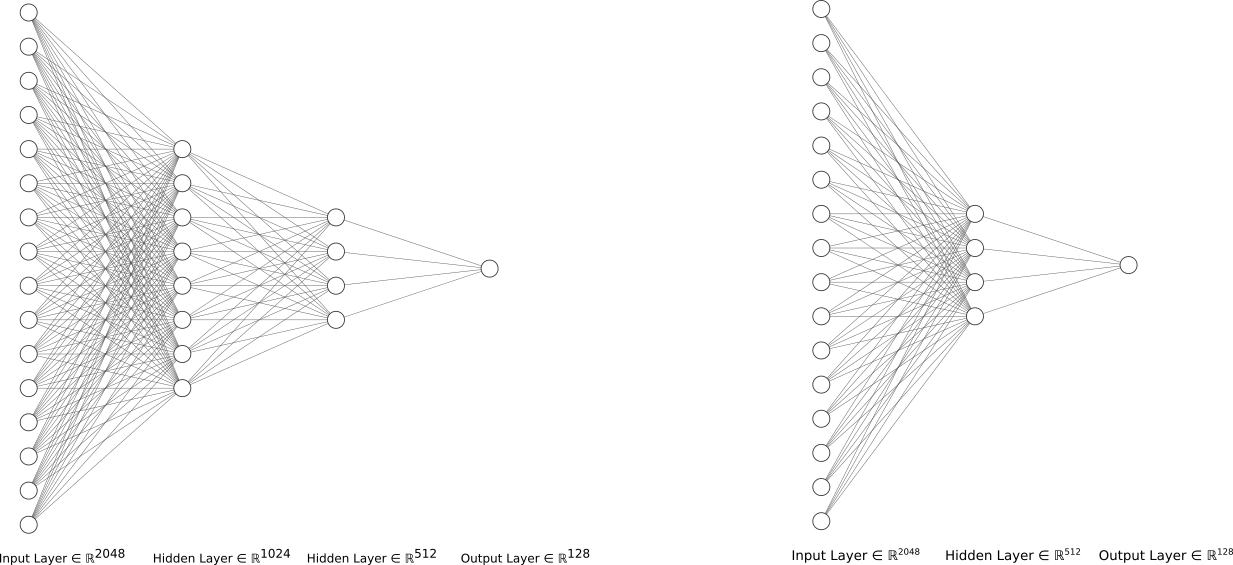
\includegraphics[width=0.8\textwidth]{Images/rl_architecture.png}
    \caption{TOBE CHANGED RL Framework Architecture: Actor-Critic Network}
    \label{fig:rlarchitecture}
\end{figure}

The \ac{RL} framework has been implemented using the \textit{Stable Baselines 3} library \cite{raffin_stable-baselines3_2021}. The \ac{RL} framework has been trained for $10$M steps, which given the episodic length, corresponds to $10$ epochs. The INSERT FIGURE below represents the main metrics collected in the training process. In particular the figure shows the mean reward, the mean episode length, the mean episodic reward, the approximated KL divergence and the explained variance.


\section{Evolutionary Algorithm Problem Definition}

The evolutionary algorithm has been used in the codesign loop to select motor parameters from a set of possible values. The evolutionary algorithm has been implemented using the \textit{DEAP} library CITE.

The motor set of parameters is composed of three main components: motor inertia, motor viscous friction and gear ratio. This choice has been made in order to keep the number of parameters low, in order to reduce the computational cost of the optimization process. The decision process is then repeated for each motor of the robot, which means that the total number of combination are:

\begin{equation}
    H = \binom{n + k - 1}{k} = \binom{23 + 3 - 1}{3} = \frac{25!}{3! 22!} = 2300
\end{equation}

where $n$ is the number of motors and $k$ is the number of parameters for each motor. In order to reduce the computational expense, we decided to focus on four crucial motors of the robot, which are the motors of the legs. This choice has been made because the legs are the main component of the robot that interacts with the environment, and therefore the choice of the motor parameters has a great impact on the performance of the robot. The total number of combinations is then reduced to:

\begin{equation}
    H = \binom{n + k - 1}{k} = \binom{4 + 3 - 1}{3} = \frac{6!}{3! 3!} = 20
\end{equation}

The evolutionary algorithm has been used to select the motor parameters from the set of possible values. The set of possible values for each parameter is shown in the \cref{tab:motorparams}.

\begin{table}[h]
    \centering
    \begin{tabular}{l c c c}
        \toprule
        \textbf{Motor} & \textsc{Inertia} $[k\mathrm{gm}^2]$ & \textsc{Gear Ratio} & \textsc{Viscous Friction} $[\mathrm{N}s\mathrm{rad}^{-1}]$ \\
        \midrule
        \textbf{S}     & $0.0001$                            & $1/100.0$           & $0.1$                                                      \\
        \textbf{M}     & $0.001$                             & $1/100.0$           & $0.15$                                                     \\
        \textbf{L}     & $0.001$                             & $1/160.0$           & $0.2$                                                      \\
        \bottomrule
    \end{tabular}
    \caption{Motor Set Parameters}
    \label{tab:motorparams}
\end{table}


After a preliminary analysis of the problem, the following parameters have been selected:

\begin{table}
    \centering
    \begin{tabular}{ll}
        \toprule
        \textbf{Parameter}    & \textbf{Value} \\
        \midrule
        Population Size       & $100$          \\
        Number of Generations & $100$          \\
        Crossover Probability & $0.5$          \\
        Mutation Probability  & $0.2$          \\
        \bottomrule
    \end{tabular}
    \caption{Evolutionary Algorithm Hyperparameters}
\end{table}

Given the single objective of the optimization problem, the \ac{NSGA}-III algorithm has been selected as the evolutionary algorithm, as it allows to find a set of solutions that are all Pareto optimal.



\section{Codesigning the Robot}

The first step of the codesign loop involves some inital design choices, which are then used to create the initial population of the evolutionary algorithm. Then the population gets evaluated running in parallel the \ac{RL} framework for each individual of the population. The evaluation process is repeated for a number of generations, after which the best individual is selected and its parameters are used to update the robot design. The process is then repeated until the robot reaches the desired target fitness or when it reaches the maximum number of generations.

For the evaluation, the reward coming from the \ac{RL} training process is used as the fitness function of the evolutionary algorithm. The fitness function is then normalized to the range $[0,1]$ in order to make the optimization more stable.

\chapter*{Epilogue}
\label{chp:99-Epilogue}

This work presented a novel framework based on the combination of reinforcement learning and evolutionary algorithms for the codesign of humanoid robots supported by hardware accelerated simulators. In particular, it answers the research question:

\begin{quote}
    \textit{
        Can humanoid robots be endowed with embodied cognition?}
\end{quote}

in which \textit{embodied cognition} refers to a synergy between the robot's hardware and the control system that makes an intelligence behavior emerge. In the scope of this thesis, the hardware is represented by the motors actuating the joints of the robot, and the control system is represented by a control policy obtained via deep reinforcement learning.
In order to answer this question, the work presents a novel framework that combines reinforcement learning and evolutionary algorithms to optimize the motor parameters of a robot with respect to a given task. In particular,

\begin{description}
    \item[In \cref{part:background}] the work presented the background knowledge required to understand the work, starting from the notation and the mathematical preliminaries of rigid multibody dynamics. The groundwork was then used to present the original formulation of the \ac{ABA} algorithm, which is the basis for the forward dynamics computation in this framework. Then, we moved to an overview of the current state of the art in the scope of hardware accelerated simulators, with a focus on the emerging role of \jax in the field of deep learning and robotics. Finally, the theoretical background of deep reinforcement learning and evolutionary algorithms was presented, introducing the reader to the main concepts of the two fields and the most common algorithms used in the literature.
    \item[In \cref{part:contributions}] the thesis proposed the two main contribution of the thesis. First, it guided the reader to the understanding of the implementation of a modified version of the \ac{ABA} algorithm that allows a holistic computation of the forward dynamics of a multibody system when there is the need to take into account the motor dynamics. Moreover, the reformulation served as an additional feature for the hardware accelerated \jaxsim simulator, allowing to consider the effect of rotors in the robot joints during simulation. As a second contribution, the thesis described the implementation of a codesign loop which creates a synergy between reinforcement learning and evolutionary algorithms in order to guide the optimization of the motor parameters of a robot, while learning a policy able to act as its control system.
\end{description}

This work addressed therefore the problem of the limited offer of simulation environments that allow for a computation of the forward dynamics that takes into account the presence of motors mounted on the joints of the robot in a hardware accelerated simulator. The framework was tested on a simple, yet easily scalable environment, and the results showed that the developed architecture is able to find a set of motor parameters that allows for a better reward in the reinforcement learning scenario.
The proposed approach for the codesign can potentially be a starting point for a further extension to the generation of new humanoid robots in which the hardware is optimized together with the control strategy. Furthermore, it could be propelled by the recent advances in the field of hardware acceleration and the development of differentiable physics engines, which is crucial for the development of a more extensive co-optimization architecture.


\chapter*{Acronyms}

% Put longest acronym in \begin{acronym}[LONGESTACRO] so that the width is fitted respect to that

\begin{acronym}[TRPO]
    \acro{ABA}{Articulated Body Algorithm}

    \acro{API}{Application Programming Interface}

    \acro{CRBA}{Composite Rigid Body Algorithm}

    \acro{CPU}{Central Processing Unit}

    \acro{CUDA}{Compute Unified Device Architecture}

    \acro{DL}{Deep Learning}

    \acro{DRL}{Deep Reinforcement Learning}

    \acro{DoF}{Degree of Freedom}

    \acro{EoM}{Equation of Motion}

    \acro{GA}{Genetic Algorithm}

    \acro{GAE}{Generalized Advantage Estimation}

    \acro{GPU}{Graphical Processing Unit}

    \acro{JIT}{Just In Time}

    \acro{MDP}{Markov Decision Process}

    \acro{MPC}{Model Predictive Control}

    \acro{NN}{Neural Network}

    \acro{NSGA}{Non-dominated Sorting Genetic Algorithm}

    \acro{PPO}{Proximal Policy Optimization}

    \acro{RBDA}{Rigid Body Dynamics Algorithm}

    \acro{ReLU}{Rectified Linear Unit}

    \acro{RL}{Reinforcement Learning}

    \acro{SDE}{State Dependent Exploration}

    \acro{SDF}{Simulation Description Format}

    \acro{TD}{Temporal Difference}

    \acro{TPE}{Tree-structured Parzen Estimator}

    \acro{TRPO}{Trust Region Policy Optimization}

    \acro{URDF}{Unified Robot Description Format}

\end{acronym}

\phantomsection

\pdfbookmark[1]{List of Symbols}{los}

\nomenclature[RL]{$\mathcal{S}$}{State Space}
\nomenclature[RL]{$\mathcal{A}$}{Action Space}
\nomenclature[RL]{$\mathcal{F} (\mathbf{s} ^\prime | \mathbf{s}, \mathbf{a}) : \mathcal{S} \time \mathcal{A} \times \mathcal{S} \rightarrow \mathbb{P}(\mathcal{S})$}{State Transition Probability}
\nomenclature[RL]{$\mathcal{R} (\mathbf{s} ^\prime | \mathbf{s}, \mathbf{a})  : \mathcal{S} \time \mathcal{A} \times \mathcal{S} \rightarrow \mathbb{R}$}{Reward Function}
\nomenclature[RL]{$\mathcal{H}$}{Hilbert Space}
\nomenclature[RL]{$\mathrm{KL}$}{Kullback-Leibler Divergence}
\nomenclature[RL]{$\gamma$ \in [0,1]}{Discount Factor}
\nomenclature[RL]{$\mathbb{P}(\cdot)$}{Probability}
\nomenclature[RL]{$\mathbb{E}(\cdot)$}{Expectation}
\nomenclature[RL]{$\hat{\mathbb{E}}(\cdot)$}{Empirical Expectation}
\nomenclature[RL]{$V (\mathbf{s})$}{State-Value Function}
\nomenclature[RL]{$A (\mathbf{s}, \mathbf{a})$}{Advantage Function}
\nomenclature[RL]{$Q (\mathbf{s}, \mathbf{a})$}{Action-Value Function}
\nomenclature[RL]{$\pi (\mathbf{a} | \mathbf{s})$}{Policy}
\nomenclature[RL]{$\pi_\theta (\mathbf{a} | \mathbf{s})$}{Policy Parametrized by $\theta$}
\nomenclature[RL]{$r _t$}{Immediate Reward at time step $t$}
\nomenclature[RL]{$a \sim \pi (\cdot | \mathbf{s})$}{Action sampled from the policy $\pi$}


\nomenclature[ROB]{$\mathrm{SO}3$}{Special Orthogonal Lie Group}
\nomenclature[ROB]{$\mathrm{SE}3$}{Special Euclidean Lie Group}
\nomenclature[ROB]{$\mathfrak{se3}$}{Lie Algebra of $SO3$}
\nomenclature[ROB]{$\mathfrak{so3}$}{Lie Algebra of $SO3$}
\nomenclature[ROB]{${}^A\mathbf{p} \in \mathbb{R}^3$}{Position Vector from A to B, measured in A}
\nomenclature[ROB]{${}^A\mathbf{R}_B \in \mathrm{SO}(3)$}{Rotation Matrix from frame B to frame A}
\nomenclature[ROB]{${}^B\mathbf{v}_A \in \mathbb{R}^3$}{Velocity Vector from A to B, measured in B}
\nomenclature[ROB]{${}^B\boldsymbol{\omega}_A \in \mathbb{R}^3$}{Angular Velocity Vector from A to B, measured in B}
\nomenclature[ROB]{${}^B\boldsymbol{\nu}_A \in \mathbb{R}^6$}{Velocity Vector from A to B, measured in A}
\nomenclature[ROB]{${}^A X _B$}{Velocity Transformation from frame B to frame A}
\nomenclature[ROB]{${}^A H_B \in \mathrm{SE}(3)$}{Homogeneous Transformation from frame B to frame A}
\nomenclature[ROB]{${}_Bf \in \mathbb{R}^3$}{Linear Force Vector, measured in B}
\nomenclature[ROB]{${}^B\tau \in \mathbb{R}^3$}{Torque Vector, measured in B}
\nomenclature[ROB]{${}_B \mathbf{f} \in \mathbb{R}^6$}{Wrench, measured in B}
\nomenclature[ROB]{$\mathbb{M} \in \mathbb{R}^{6 \times 6}$}{Inertia Matrix}
\nomenclature[ROB]{$g \in \mathbb{R}^+$}{Gravity Acceleration Constant}
\nomenclature[ROB]{$\mathbf{g} \in \mathbb{R}^3$}{Gravity Vector}
\nomenclature[ROB]{$n \in \mathbb{N}$}{Number of Degrees of Freedom}
\nomenclature[ROB]{$\boldsymbol{\Phi}_i \in \mathbb{R}^{6}$}{Joint Motion Subspace for a joint $i$}
\nomenclature[ROB]{$\mathbf{s} \in \mathbb{R}^n$}{Joint Position Vector}
\nomenclature[ROB]{$\dot{\mathbf{s}} \in \mathbb{R}^n$}{Joint Velocity Vector}
\nomenclature[ROB]{$\ddot{\mathbf{s}} \in \mathbb{R}^n$}{Joint Acceleration Vector}
\nomenclature[ROB]{$\mathbf{h} \in \mathbb{R}^{6+n}$}{Coriolis Vector}
\nomenclature[ROB]{$q \in \mathbb{H} : \lVert q \rVert = 1$}{Unit Quaternion}
\nomenclature[ROB]{$\lambda (i)$}{Parent link of link $i$}


\nomenclature[MATH]{$\mathbb{I}$}{Identity Matrix}
\nomenclature[MATH]{$\mathbbm{0} _n$}{Null Squared Matrix of size $n$}
\nomenclature[MATH]{$\mathbbm{1} _n$}{All-Ones Squared Matrix of size $n$}
\nomenclature[MATH]{$\times$}{Cross Product}
\nomenclature[MATH]{$\lVert \cdot \rVert _\mathcal{F} \equiv \lVert \cdot \rVert _{\ell ^2}$}{Frobenius Norm or $\ell ^1$ Norm}

\renewcommand{\nomname}{List of Symbols}
\printnomenclature
%-------------------------------------------------------------------------
%	BIBLIOGRAPHY
%-------------------------------------------------------------------------

\addtocontents{toc}{\vspace{2em}} % Add a gap in the Contents, for aesthetics
\bibliography{references}

%-------------------------------------------------------------------------
%	APPENDICES
%-------------------------------------------------------------------------

\cleardoublepage
\addtocontents{toc}{\vspace{2em}} % Add a gap in the Contents, for aesthetics
\appendix
\chapter{Appendix A}
If you need to include an appendix to support the research in your thesis, you can place it at the end of the manuscript.
An appendix contains supplementary material (figures, tables, data, codes, mathematical proofs, surveys, \dots)
which supplement the main results contained in the previous chapters.

\chapter{Appendix B}
It may be necessary to include another appendix to better organize the presentation of supplementary material.


% LIST OF FIGURES
\listoffigures

% LIST OF TABLES
\listoftables

% LIST OF SYMBOLS
% Write out the List of Symbols in this page
% \chapter*{List of Symbols} % You have to include a chapter for your list of symbols (
% \begin{table}[H]
%     \centering
%     \begin{tabular}{lll}
%         \textbf{Variable} & \textbf{Description} & \textbf{SI unit} \\\hline\\[-9px]
%         $\bm{u}$ & solid displacement & m \\[2px]
%         $\bm{u}_f$ & fluid displacement & m \\[2px]
%     \end{tabular}
% \end{table}

% ACKNOWLEDGEMENTS
\chapter*{Acknowledgements}
Here you might want to acknowledge someone.


\cleardoublepage

\end{document}
